\documentclass[11pt,a4paper]{report}

% ---------------- Packages ----------------
\usepackage[margin=1in]{geometry}
\usepackage{graphicx}
\usepackage{amsmath}
\usepackage{booktabs}
\usepackage{array}
\usepackage{tabularx}
\usepackage{enumitem}
\usepackage{xcolor}
\usepackage{titlesec}
\usepackage{float}
\usepackage{tikz}
\usetikzlibrary{shapes.geometric, arrows.meta, positioning, calc}
\usepackage[hidelinks]{hyperref}
\usepackage{url}

% ---------------- Chapter style: "Chapter 1 Abstract" ----------------
\titleformat{\chapter}[hang]{\Huge\bfseries}{Chapter \thechapter}{0.5em}{}
\titlespacing*{\chapter}{0pt}{0pt}{25pt}

% ---------------- Helper: red placeholder for values you must fill ----------------
\newcommand{\tbd}[1]{\textcolor{red}{#1}}

\setlength{\parindent}{0pt}
\setlength{\parskip}{6pt}
\renewcommand{\arraystretch}{1.15}

\begin{document}

% =====================================================
%                    TITLE PAGE
% =====================================================
\begin{titlepage}
\thispagestyle{empty}
\begin{tikzpicture}[remember picture, overlay]
  \draw[line width=0.8pt]
    ($(current page.north west)+(1.6cm,-1.6cm)$) rectangle
    ($(current page.south east)+(-1.6cm,1.6cm)$);
\end{tikzpicture}

\centering
\vspace*{1.5cm}

% Put the university logo file in the same folder as this .tex file
% and name it jklu_logo.png (or change the name below).
\IfFileExists{jklu_logo.png}{\includegraphics[width=0.28\textwidth]{jklu_logo.png}}{\fbox{\parbox{3cm}{\centering\vspace{1cm}JKLU Logo\vspace{1cm}}}}

\vspace{1.5cm}

{\large\bfseries Institute of Engineering and Technology (IET)}\\[0.4cm]
{\large\bfseries Major Project End-Semester Report}\\[1cm]

{\Huge\bfseries Intelligent Academic \& Career\\ Copilot}\\[0.4cm]
{\huge\bfseries (RAG + ML)}\\[1cm]

{\bfseries Project Code: PR1107}\\[1cm]

{\bfseries Submitted By}\\[0.2cm]
{\bfseries Nakul Ranka} (2023BTech050)\\
{\bfseries Prateek Goswami} (2023BTech058)\\
{\bfseries Siddharth Ranka} (2023BTech082)\\[1.2cm]

{\bfseries Faculty Guide}\\[0.1cm]
{\bfseries Prof. Devendra Bhavsar}\\
Institute of Engineering and Technology, JKLU\\[1.5cm]

{\bfseries November 2026}
\end{titlepage}

% =====================================================
%                    CONTENTS
% =====================================================
\pagenumbering{roman}
\setcounter{page}{1}

\tableofcontents
\clearpage
\listoftables
\clearpage
\listoffigures
\clearpage

\pagenumbering{arabic}
\setcounter{page}{1}

% =====================================================
%                    1. ABSTRACT
% =====================================================
\chapter{Abstract}

Engineering students often face a gap between university examinations and technical job interviews. Existing study aids and general-purpose LLM chatbots are one-directional, do not know the student's syllabus, and give no numbers about conceptual weaknesses.

This project presents the \textbf{Intelligent Academic \& Career Copilot}, which combines Retrieval-Augmented Generation (RAG) with supervised Machine Learning. The platform reads syllabi, lecture notes, slide decks, past papers and student resumes, answers questions based on them, and conducts adaptive mock technical interviews matched to a target Job Description (JD).

A Hybrid Retrieval Engine merges BM25 keyword matching with dense Sentence-Transformer embeddings using Reciprocal Rank Fusion (RRF). A Cross-Encoder reranker, query decomposition and HyDE further improve the quality of retrieved passages. Interview answers are scored on six dimensions (semantic accuracy, latency, length, keyword coverage, confidence and completeness) by a VotingRegressor ensemble of Random Forest and XGBoost, which reached an RMSE of about 0.06 and an $R^2$ of about 0.93.

The main contribution is a closed-loop remediation engine: when a topic score falls below 70\%, the system retrieves matching passages from the student's own notes, builds a study plan, and generates targeted re-tests. In the final phase we added spoken interviews using Whisper and multi-user login with JWT. The whole system runs on a zero-cost stack of open-weight models, CPU embeddings, FastAPI and Streamlit.

% =====================================================
%                    2. INTRODUCTION
% =====================================================
\chapter{Introduction}

Moving from undergraduate coursework to professional software and data roles needs both strong academic understanding and the ability to explain ideas clearly in technical interviews. Students find it hard to combine syllabi, slides and textbooks into effective preparation. Generic AI tools help only partly:

\begin{enumerate}
  \item \textbf{No course context:} general LLMs may make up facts and do not know the student's syllabus or lecture notes.
  \item \textbf{Passive use:} they answer questions but do not test whether the student has really learned the material.
  \item \textbf{No quantitative diagnostics:} latency, keyword coverage and topic-wise scores (for example, SQL: 61\%) are not measured.
  \item \textbf{Broken feedback loop:} a failed answer is never linked back to the relevant slide in the student's notes.
\end{enumerate}

The copilot addresses these gaps through four modules:

\begin{enumerate}
  \item \textbf{Document Intelligence} for multi-format upload and structure-aware chunking.
  \item \textbf{RAG Assistant} for grounded question answering using hybrid BM25 + dense search and reranking.
  \item \textbf{AI Interviewer} for resume--JD skill-gap matching across 12+ disciplines and stateful mock interviews (typed or spoken).
  \item \textbf{ML Scoring \& Adaptive Loop} for answer scoring, weakness diagnosis and study guides linked to the student's notes.
\end{enumerate}

This report describes the full work done in the project, from design to final implementation, along with the results obtained and the lessons learned.

% =====================================================
%                    3. PROBLEM STATEMENT
% =====================================================
\chapter{Problem Statement}

Students preparing for exams and campus placements face four main problems:

\begin{enumerate}
  \item \textbf{No curricular grounding.} Question banks (LeetCode, GeeksforGeeks, AmbitionBox) ignore the depth and terms of a given syllabus, while chatbots give generic explanations that may differ from lecture material.
  \item \textbf{Passive interaction.} Active recall and viva-style questioning are missing, which leads to an ``illusion of competence''.
  \item \textbf{No multi-dimensional objective scoring.} Platforms use binary unit tests or subjective LLM grading instead of measuring semantic accuracy, latency, keyword coverage and confidence.
  \item \textbf{No closed-loop remediation.} Software stops once a test is graded. It does not find the weak topic, fetch the student's own notes, suggest revision time and re-test.
\end{enumerate}

\textbf{Formal objective.} To design, develop and validate an intelligent academic and career copilot that uses hybrid RAG (BM25 + dense vectors) and supervised ensemble ML (Random Forest + XGBoost) to read academic documents, conduct resume- and JD-aligned technical interviews, score responses on multiple metrics, and close the learning gap through an automated remediation and re-testing loop.

\section{Objectives}
\begin{itemize}
  \item Design a system to process and store documents for quick retrieval.
  \item Build a RAG pipeline that answers questions from uploaded documents with citations.
  \item Develop an AI interviewer that generates and conducts practice interviews.
  \item Create an ML model that analyses student performance and finds weak topics.
  \item Implement an adaptive learning loop that recommends study material and re-tests the student.
  \item Improve the RAG pipeline using hybrid retrieval and reranking strategies.
\end{itemize}

% =====================================================
%                    4. DATASET
% =====================================================
\chapter{Dataset}

\begin{enumerate}
  \item \textbf{Academic document corpus.} Syllabi, slides, assignments and past papers in \texttt{.pdf}, \texttt{.docx}, \texttt{.pptx}, \texttt{.txt} and \texttt{.md} formats are parsed with PyPDF2, python-docx and python-pptx. Each chunk carries metadata: \texttt{chunk\_id} (UUIDv4), \texttt{source\_file}, \texttt{doc\_type} (syllabus, notes, resume, exam), \texttt{section\_title}, \texttt{page\_number} and \texttt{chunk\_index}. Chunking is heading-aware with a 512-word window and 64-word overlap.

  \item \textbf{Interview question bank.} The bank started with 40+ verified questions collected from AmbitionBox, GeeksforGeeks and interview records. In the final phase, live scrapers and automatic deduplication expanded it to {200+} questions across {15} domains. Each entry stores \texttt{question\_id}, \texttt{topic}, \texttt{difficulty}, \texttt{question}, \texttt{reference\_answer} and \texttt{expected\_keywords}. Table~\ref{tab:qbank} shows the composition of the initial bank.

  \item \textbf{Synthetic response dataset.} 500 feature-engineered vectors in five quality tiers: Excellent (0.85--1.00), Good (0.70--0.84), Average (0.50--0.69), Poor (0.30--0.49) and Bad (0.00--0.29). It trains the VotingRegressor before real student data is available.

\end{enumerate}

\begin{table}[H]
\centering
\begin{tabular}{lclc}
\toprule
\textbf{Domain} & \textbf{Qs} & \textbf{Domain} & \textbf{Qs}\\
\midrule
Python Core & 7 & SQL \& Databases & 6\\
Data Structures \& Algorithms & 6 & System Design & 4\\
Machine Learning Theory & 7 & Natural Language Processing & 4\\
Deep Learning & 4 & Data Science Principles & 2\\
Computer Vision & 1 & & \\
\bottomrule
\end{tabular}
\caption{Initial question bank composition.}
\label{tab:qbank}
\end{table}

% =====================================================
%                    5. SYSTEM ARCHITECTURE
% =====================================================
\chapter{System Architecture}

The copilot has five layers for modularity and zero-cost local execution (Figure~\ref{fig:arch}).

\begin{figure}[H]
\centering
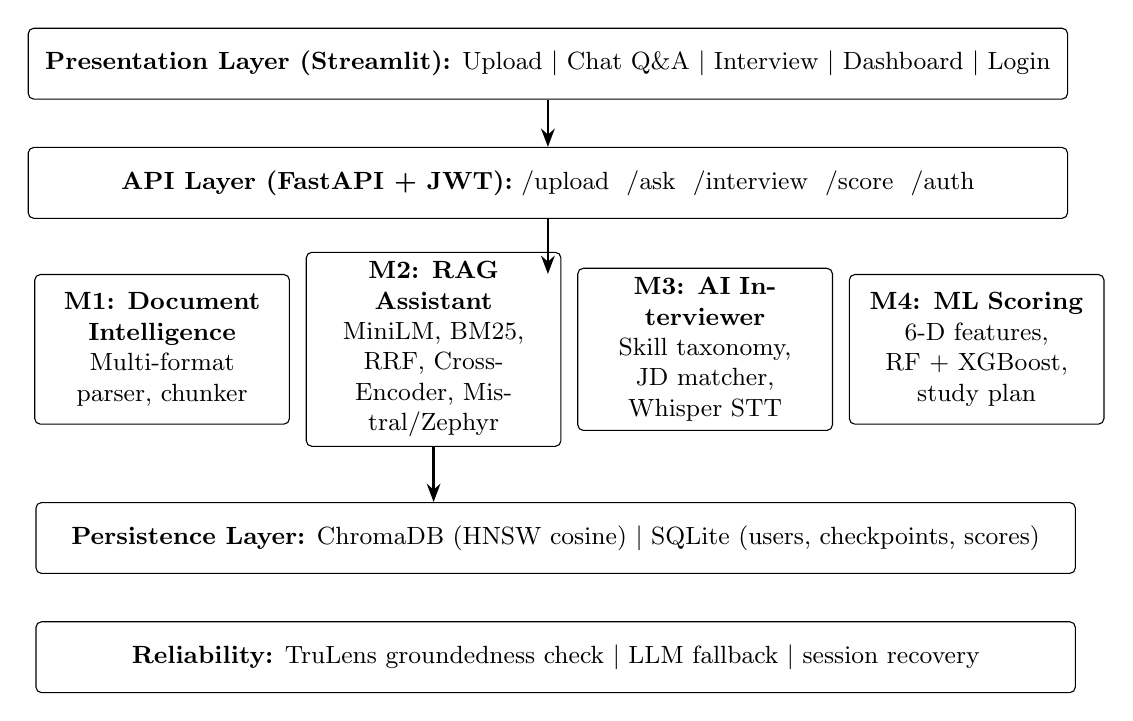
\begin{tikzpicture}[
  box/.style={draw, rounded corners=2pt, align=center, minimum height=0.9cm, font=\small},
  wide/.style={box, minimum width=13.2cm},
  mod/.style={box, minimum width=3.1cm, minimum height=1.9cm, text width=3.0cm},
  arr/.style={-{Stealth}, thick}
]
\node[wide] (ui) {\textbf{Presentation Layer (Streamlit):} Upload $|$ Chat Q\&A $|$ Interview $|$ Dashboard $|$ Login};
\node[wide, below=0.6cm of ui] (api) {\textbf{API Layer (FastAPI + JWT):} /upload \ /ask \ /interview \ /score \ /auth};

\node[mod, below=0.7cm of api, xshift=-4.9cm] (m1) {\textbf{M1: Document Intelligence}\\ Multi-format parser, chunker};
\node[mod, right=0.2cm of m1] (m2) {\textbf{M2: RAG Assistant}\\ MiniLM, BM25, RRF, Cross-Encoder, Mistral/Zephyr};
\node[mod, right=0.2cm of m2] (m3) {\textbf{M3: AI Interviewer}\\ Skill taxonomy, JD matcher, Whisper STT};
\node[mod, right=0.2cm of m3] (m4) {\textbf{M4: ML Scoring}\\ 6-D features, RF + XGBoost, study plan};

\node[wide, below=0.7cm of m2, xshift=1.55cm] (db) {\textbf{Persistence Layer:} ChromaDB (HNSW cosine) $|$ SQLite (users, checkpoints, scores)};
\node[wide, below=0.6cm of db] (ev) {\textbf{Reliability:} TruLens groundedness check $|$ LLM fallback $|$ session recovery};

\draw[arr] (ui) -- (api);
\draw[arr] (api) -- ($(api.south)+(0,-0.7cm)$);
\draw[arr] (m2.south) -- ($(m2.south)+(0,-0.7cm)$);
\end{tikzpicture}
\caption{High-level architecture of the copilot.}
\label{fig:arch}
\end{figure}

\section{Execution Flow}
\begin{enumerate}
  \item \textbf{Ingestion:} upload $\rightarrow$ parse $\rightarrow$ 512-word chunks $\rightarrow$ MiniLM embeddings stored in ChromaDB and the BM25 index.
  \item \textbf{Q\&A:} query decomposition / HyDE $\rightarrow$ BM25 and dense search $\rightarrow$ RRF merge $\rightarrow$ Cross-Encoder rerank $\rightarrow$ top chunks injected into the Mistral-7B prompt $\rightarrow$ cited answer.
  \item \textbf{Interview:} resume + JD $\rightarrow$ skill-gap matching $\rightarrow$ 10 difficulty-mixed questions with a countdown timer. Answers can be typed or spoken (Whisper speech-to-text).
  \item \textbf{Scoring:} six features $\rightarrow$ VotingRegressor score (0--1) and grade $\rightarrow$ SQLite checkpoint $\rightarrow$ topic averages updated.
  \item \textbf{Adaptive loop:} topics below 70\% $\rightarrow$ retrieve the student's notes $\rightarrow$ study plan and re-test questions $\rightarrow$ Plotly dashboard.
\end{enumerate}

% =====================================================
%                    6. IMPLEMENTATION
% =====================================================
\chapter{Implementation}

The repository contains about {40} files and over {6,500} lines of modular Python code. This chapter explains the design choices and the final implementation of each part.

\section{Research and Design Decisions}

\textbf{Retrieval.} Dense-only retrieval was found to dilute technical acronyms such as PCA, ACID, GIL, BFS and DAG. So a hybrid pipeline with weighted RRF was used:
\begin{equation}
  \mathrm{RRF}(d) = \frac{0.4}{60 + \mathrm{rank}_{\mathrm{BM25}}(d)} + \frac{0.6}{60 + \mathrm{rank}_{\mathrm{Dense}}(d)}
  \label{eq:rrf}
\end{equation}

\textbf{Cost and latency.} Generation uses the Hugging Face Serverless Inference API (Mistral-7B-Instruct-v0.3) with a Zephyr-7B-beta fallback. Embeddings use the CPU-based \texttt{all-MiniLM-L6-v2} model (384 dimensions). Local inference with Ollama (Mistral-7B Q4\_K\_M) is available as an option.

\textbf{Skill taxonomy.} A taxonomy of 12 domains and 100+ keywords (regex word-boundary matching) with profiles for 8 roles, from ML Engineer to Software Engineer.

\textbf{Scoring model.} Six features are used instead of subjective LLM grading (Table~\ref{tab:features}).

\begin{table}[H]
\centering
\begin{tabularx}{\textwidth}{lX}
\toprule
\textbf{Feature} & \textbf{Description}\\
\midrule
Semantic similarity & Cosine similarity with the reference answer (weight 0.40)\\
Latency & Curve based on response time (5 s = 0.9, 30 s = 0.85, 60 s = 0.75, 120 s = 0.40)\\
Length & Bell-shaped word-length curve peaking at 30--120 words\\
Keyword coverage & Share of expected keywords present in the answer\\
Confidence & Assertive words versus hedge words\\
Completeness & Share of complete, well-formed sentences\\
\bottomrule
\end{tabularx}
\caption{The six scoring features.}
\label{tab:features}
\end{table}

\section{Backend}

The FastAPI backend has four modules and an API layer:

\begin{itemize}
  \item \textbf{Document Intelligence:} \texttt{parser.py} (PDF/DOCX/PPTX/TXT/MD with graceful handling of corrupt pages) and \texttt{chunker.py} (heading- and slide-aware, UUID-tagged chunks).
  \item \textbf{RAG Assistant:} \texttt{embeddings.py} (L2-normalized CPU batches), \texttt{hybrid\_retriever.py} (ChromaDB + BM25Okapi, RRF, metadata filters, index sync), \texttt{reranker.py} (Cross-Encoder), \texttt{query\_tools.py} (query decomposition and HyDE) and \texttt{generator.py} (prompting, citations, dual-model fallback).
  \item \textbf{AI Interviewer:} \texttt{role\_matcher.py} (skill-gap sets), \texttt{question\_generator.py} (25\% Easy, 50\% Medium, 25\% Hard), \texttt{scraper\_pipeline.py} (live scrapers with deduplication) and \texttt{speech.py} (Whisper speech-to-text).
  \item \textbf{ML Scoring:} \texttt{feature\_extractor.py}, \texttt{model.py} (RF + XGBoost VotingRegressor) and \texttt{recommendation\_engine.py} (weak topics below 70\%; Critical below 40\%, Moderate 40--60\%, Mild 60--70\%; study plans with estimated hours; RAG note retrieval).
  \item \textbf{API and utilities:} routes for upload, ask, interview, score and auth; \texttt{auth.py} (JWT login and per-user data isolation); \texttt{checkpoint.py} (SQLite state recovery) and \texttt{logger.py}.
\end{itemize}

\section{Advanced Retrieval Components}

\begin{itemize}
  \item \textbf{Cross-Encoder reranker.} The top results from RRF are rescored by the \texttt{ms-marco-MiniLM-L-6-v2} cross-encoder, which reads the query and the passage together. This gives a more accurate ordering than comparing separate embeddings.
  \item \textbf{Query decomposition.} A long or multi-part question (for example, ``Compare PCA and LDA'') is split into simple sub-questions. Each is searched separately and the results are merged.
  \item \textbf{HyDE (Hypothetical Document Embeddings).} For very short or vague queries, the LLM first writes a short imaginary answer. This answer is embedded and used for dense search, which often matches the real notes better than the short query.
\end{itemize}

\section{Speech-to-Text Interviews}

To feel more like a real interview, students can answer by speaking. The audio is converted to text by OpenAI Whisper and then passed through the same six-feature scoring pipeline. The speaking time is also used as the latency feature.

\section{Authentication and Data Isolation}

Multiple students can now use the same system. Users register and log in, and the server returns a JWT token. Every upload, chat history, interview result and score is stored with the user's ID, and the vector store is filtered by this ID so that one student can never see another student's notes.

\section{Frontend}

A multi-page Streamlit app with custom CSS and Plotly charts:

\begin{itemize}
  \item \textbf{Login view:} register and sign in.
  \item \textbf{Upload view:} drag-and-drop uploader, document type selector, indexing progress bar and indexed-file history.
  \item \textbf{Chat view:} curriculum Q\&A with collection, document type and \texttt{top\_k} controls. Answers show expandable citations (file, page/slide, confidence).
  \item \textbf{Interview view:} setup wizard (role, resume, JD, level, question count), live timer, progress bar, a microphone option, and per-question score (0--100\%) with grade (A+ to F). It also has early exit and a summary card.
  \item \textbf{Dashboard:} skill radar chart, topic bar chart with a 70\% threshold line, severity badges, a personalized study plan with excerpts from the student's notes, an adaptive re-test plan, and a demo mode with sample data.
\end{itemize}

\section{Project Timeline Summary}

\begin{table}[H]
\centering
\begin{tabularx}{\textwidth}{lXX}
\toprule
\textbf{Week} & \textbf{Work Done} & \textbf{Deliverable}\\
\midrule
Weeks 1--6 & Research, document pipeline, hybrid retrieval, interviewer, ML scoring, Streamlit UI & Working prototype (mid-term)\\
Week 7 & Live scrapers for AmbitionBox and GeeksforGeeks; question deduplication & Expanded question bank\\
Week 8 & Cross-Encoder reranker; query decomposition and HyDE & Reranker pipeline\\
Week 9 & Whisper speech-to-text; JWT authentication & Spoken interviews; per-user data\\
Week 10 & Testing and documentation & Final report, demo video, defense\\
\bottomrule
\end{tabularx}
\caption{Summary of the project timeline.}
\end{table}

% =====================================================
%                    7. RESULTS
% =====================================================
\chapter{Results}

\section{ML Scoring Model}

The VotingRegressor (Random Forest + XGBoost) was trained on the 500-sample synthetic dataset and tested on a held-out set. Table~\ref{tab:ml} shows the results.

\begin{table}[H]
\centering
\begin{tabular}{lc}
\toprule
\textbf{Metric} & \textbf{Value}\\
\midrule
RMSE & $\approx 0.06$\\
MAE & $\approx 0.05$\\
$R^2$ & $\approx 0.93$\\
\bottomrule
\end{tabular}
\caption{Performance of the scoring model.}
\label{tab:ml}
\end{table}

A low RMSE and a high $R^2$ show that the six features explain the answer quality well and that the ensemble predicts scores close to the target values. The ensemble was more stable than either model alone.

\section{Adaptive Loop Demonstration}

A sample run shows how the closed loop works. A student scoring SQL: 61\% is marked as a Mild weak topic. The system retrieves the matching slides from the student's own DBMS notes, creates a study plan with estimated hours, and generates new SQL questions for a re-test. After revision, the new score is saved and the dashboard is updated.

\begin{figure}[H]
\centering
\includegraphics[width=0.9\textwidth]{screenshot1.png}
\caption{Dashboard interface}
\label{fig:demo1}
\end{figure}

\begin{figure}[H]
\centering
\includegraphics[width=0.9\textwidth]{screenshot2.png}
\caption{Interface showing ATS score and actionable revision guidance}
\label{fig:demo2}
\end{figure}

\begin{figure}[H]
\centering
\includegraphics[width=0.9\textwidth]{screenshot3.png}
\caption{Interface showing diagnosis}
\label{fig:demo3}
\end{figure}

Figures~\ref{fig:demo1} ,~\ref{fig:demo2} and~\ref{fig:demo3} show the dashboard, diagnosis and ATS score and actionable revision guidance.

% =====================================================
%                    8. CHALLENGES
% =====================================================
\chapter{Challenges and Solutions}

\begin{enumerate}
  \item \textbf{API rate limits and cold starts} (10--30 s delays on the free tier). \emph{Solution:} Mistral-7B $\rightarrow$ Zephyr-7B failover and optional local Ollama inference.
  \item \textbf{Scanned or complex documents} cannot be parsed cleanly by PyPDF2. \emph{Solution:} graceful per-page degradation; OCR (Tesseract/Surya) is left as future work.
  \item \textbf{Scarce real answer data.} \emph{Solution:} a 500-sample synthetic training set and an active-learning log that adds real interactions over time.
  \item \textbf{Latency in real-time interviews.} \emph{Solution:} asynchronous CPU feature extraction with cached embeddings; SQLite checkpoints save progress when a student disconnects.
  \item \textbf{Hallucinated answers.} \emph{Solution:} strictly grounded prompts that require citations, and TruLens groundedness checks that reject poorly supported answers.
  \item \textbf{Web scraping changes.} Websites change their layout and may limit requests. \emph{Solution:} polite request delays, simple parsers that are easy to update, and a saved local copy of the question bank.
\end{enumerate}

% =====================================================
%                    9. CONCLUSION
% =====================================================
\chapter{Conclusion and Future Work}

\section{Conclusion}

In this project we built an Intelligent Academic \& Career Copilot that goes beyond a simple question-answering tool. It reads a student's own documents, answers questions with citations, conducts resume- and JD-based mock interviews, scores answers on six measurable features, and then uses the student's own notes to build a study plan and re-test them. The hybrid retrieval pipeline with reranking handles technical terms better than dense-only search, and the ensemble model achieved an RMSE of about 0.06 and $R^2$ of about 0.93. The final system supports spoken interviews and multiple users, and it runs entirely on free and open-source tools.

All objectives listed in the synopsis were achieved: document processing, a RAG pipeline, an AI interviewer, an ML model for weak-area prediction, and an adaptive learning loop.

\section{Limitations}
\begin{itemize}
  \item The scoring model was trained on synthetic data, so it needs real student answers for better accuracy.
  \item Scanned PDFs and handwritten notes are not yet supported.
  \item The free-tier LLM API can be slow during busy hours.
  \item The question bank is limited to the domains collected so far.
\end{itemize}

\section{Future Work}
\begin{itemize}
  \item Retrain the model on real student interactions collected through the active-learning log.
  \item Add OCR support for scanned and handwritten documents.
  \item Support more languages and more roles and domains.
  \item Add a mobile-friendly interface and progress tracking over weeks.
  \item Use a fine-tuned small language model for faster local responses.
\end{itemize}

% =====================================================
%                    10. REFERENCES
% ====================================================

\begin{thebibliography}{99}
\bibitem{lewis} P. Lewis et al., ``Retrieval-Augmented Generation for Knowledge-Intensive NLP Tasks,'' \emph{NeurIPS}, vol. 33, pp. 9459--9474, 2020. \url{https://arxiv.org/abs/2005.11401}
\bibitem{sbert} N. Reimers and I. Gurevych, ``Sentence-BERT: Sentence Embeddings using Siamese BERT-Networks,'' \emph{EMNLP-IJCNLP}, pp. 3982--3992, 2019. \url{https://arxiv.org/abs/1908.10084}
\bibitem{bm25} S. Robertson, H. Zaragoza, et al., ``The Probabilistic Relevance Framework: BM25 and Beyond,'' \emph{Found. Trends Inf. Retr.}, vol. 3, no. 4, pp. 333--389, 2009.
\bibitem{rrf} G. V. Cormack, C. L. Clarke, and S. Buettcher, ``Reciprocal Rank Fusion outperforms Condorcet and individual Rank Learning Methods,'' \emph{SIGIR '09}, pp. 758--759, 2009.
\bibitem{xgb} T. Chen and C. Guestrin, ``XGBoost: A Scalable Tree Boosting System,'' \emph{KDD '16}, pp. 785--794, 2016. \url{https://arxiv.org/abs/1603.02754}
\bibitem{rf} L. Breiman, ``Random Forests,'' \emph{Machine Learning}, vol. 45, no. 1, pp. 5--32, 2001.
\bibitem{mistral} A. Q. Jiang et al., ``Mistral 7B,'' 2023. \url{https://arxiv.org/abs/2310.06825}
\bibitem{llama} Meta AI, ``Introducing Meta Llama 3: The Most Capable Openly Available LLM to Date,'' Meta AI Research Blog, 2024.
\bibitem{hyde} L. Gao, X. Ma, J. Lin, and J. Callan, ``Precise Zero-Shot Dense Retrieval without Relevance Labels (HyDE),'' 2022. \url{https://arxiv.org/abs/2212.10496}
\bibitem{whisper} A. Radford et al., ``Robust Speech Recognition via Large-Scale Weak Supervision (Whisper),'' 2022. \url{https://arxiv.org/abs/2212.04356}
\bibitem{msmarco} R. Nogueira and K. Cho, ``Passage Re-ranking with BERT,'' 2019. \url{https://arxiv.org/abs/1901.04085}
\bibitem{chroma} Chroma Core Team, ``Chroma: The AI-native open-source embedding database,'' 2023. \url{https://github.com/chroma-core/chroma}
\bibitem{trulens} TruEra Team, ``TruLens: Open-source evaluation and tracking for LLM applications,'' 2023. \url{https://www.trulens.org/}
\bibitem{fastapi} S. Ramirez, ``FastAPI,'' 2018. \url{https://fastapi.tiangolo.com/}
\bibitem{streamlit} Streamlit Inc., ``Streamlit: A faster way to build and share data apps,'' 2023. \url{https://streamlit.io/}
\end{thebibliography}

\end{document}